\documentclass[./thesis.tex]{subfiles}

\newcommand{\minDetInT}{\text{minDetInT1}}
\newcommand{\Nteeth}{N_\text{teeth}}
\newcommand{\lTeethI}{\text{lTeethI}}

\begin{document}

\section{$\EPT$ \textit{vs} selection}

The selection of determinants and the calculation of $\EPT$, all approximations aside, both imply the computation of $\epsilon(\alpha)$ for all $\ket \alpha$, so both can be computed at the same time. The selection is about identifying the set of the most important contributions, $\EPT$ is about computing the sum over all of them. There are two main consequences to this:
\paragraph{$\EPT$ is one iteration behind the selection}
At iteration $n$, identifying the most significant $\ket \alpha$ is about building $\Psi^{n+1}$ while summing the contributions is about estimating the cost of truncation for $\Psi^{n}$. Computing $\EPT$ for a "final" wavefunction therefore requires an extra iteration, which applies to a larger number of determinants and thus is more expensive. Note that if only $\EPT$ is required, a more efficient algorithm can be used.\cite{Cimiraglia_1996}

\paragraph{The selection can take more approximations}
The computation of the sum has to be more costly than just identifying the largest terms. As was said in chapter~\ref{chap:CIPSI}, the CIPSI algorithm can take pretty drastic approximations for the selection.\cite{Evangelisti_1983}
	\begin{itemize}
		\item{$t_g$}
		allows to explore a reduced subset of $\ket \alpha$ in which we are almost sure to find those of interest.
		\item{$t_s < t_g$}
		allows for a less accurate and less expensive computation of $\epsilon(\alpha)$, which is unlikely to significantly change the identified set.
	\end{itemize}
	These approximations do not apply when computing $\EPT$. The very large number of smaller contributions makes them impossible to neglect without introducing a bias, and increasing the $t_g$ and $t_s$ thresholds dramatically increases the computational cost.


Unfortunately, a partial computation of $\EPT$ always results in a biased result. Since $\epsilon(\alpha)$ is an energy contribution, it is necessarily negative, and $\EPT$ is a sum of same-sign contributions. Therefore, when $\EPT$ is truncated some correlation energy is missing but there is little clue how much exactly. The $t_g$ and $t_s$ thresholds used in CIPSI can be seen as ways of adjusting this truncation for a given computational cost.

Before the stochastic computation of $\EPT$ was implemented, our best choice was to set low $t_g$ and $t_s$ thresholds while performing the selection, and accept very approximate values for $\EPT$ for intermediate wavefunctions. Then, once the selection was completed, we would raise them just for a final, very expensive ``$\EPT$ only'' iteration. In fact, an exact computation with $t_g=\Ngen$ and $t_s=\Ndet$ was often prohibitively long, so the final $\EPT$ was still biased, and the biases were not well controlled. The effect was particularly important when computing atomization energies, where the $\EPT$ values were much larger on the molecule than on the atoms.
A practical way to circumvent this problem was already proposed 20 years ago, by giving an extrapolation of $\EPT$ when $t_g$ goes to zero.\cite{Angeli_1997} However, the algorithm we propose here has the advantage of giving an unbiased result within a statistical confidence interval.

\section{Stochastic estimation of $\EPT$}

We eventually solved the previously discussed problem by turning the bias into an error bar. The basic idea is that, instead of trying to get the largest possible chunk of contribution, we can randomly pick $\epsilon(\alpha)$ contributions and make a Monte-Carlo estimate for the sum over all $\ket \alpha$. In this case, to avoid any bias we must set
\begin{equation}
t_g = \Ngen \; ; \; t_s = \Ndet.
\end{equation}
\alert{Verifier $t_g = 0$}.

Not only the estimate will be unbiased and much closer to the actual $\EPT$, but we will have an estimate for the error. Because $\EPT$ is itself used as an approximation
\begin{equation}
\Evar + \EPT \simeq \EFCI
\end{equation}
An error significantly smaller than the typical accuracy of $\Evar + \EPT$ \textit{vs} $\EFCI$ is certainly acceptable.


The actual Monte-Carlo computation is significantly more convoluted than simply drawing random $\kalpha$.

\paragraph{$\epsilon(\alpha)$ are packed into elementary contributions $e_I$}
Individual $\epsilon(\alpha)$ are expensive to compute. In the CIPSI algorithm, each generator determinant creates a number of unique $\kalpha$, and computes $\epsilon(\alpha)$ for each one of them.
Essentially, the set of $\kalpha$ can be grouped in $\Ngen$ disjoint sets, each associated with a generator determinant, as shown in figure \ref{fig:mu_sample}.
\begin{equation}
\epsilon(\alpha) \in \mathcal{A}_I \; ; \; \Hij{\alpha}{I} \neq 0 \; ; \;   \forall J < I, \Hij{\alpha}{J} = 0.
\end{equation}
Because of the numerous tricks described in chapter~\ref{chap:CIPSI}, we are able to compute all the $\epsilon(\alpha)$ of a set considerably faster than if we had to compute each contribution separately. Therefore, in order to access a larger chunk of data, the stochastic PT2 algorithm will not consider individual $\epsilon(\alpha)$, but instead sums of all $\epsilon(\alpha)$ from the same set:
\begin{equation}
e_I = \sum_{\alpha \in \mathcal{A}_I} \epsilon(\alpha)
\end{equation}
Indeed
\begin{equation}
\EPT = \sum_{I} e_I
\end{equation}

The $e_I$'s are already explicitly computed by our CIPSI implementation, which returns the aggregated values of $\epsilon(\alpha)$ for one task, one task being essentially associated with a generator determinant.

\paragraph{The $e_I$'s can be stored to avoid re-computation}
Each elementary contribution is associated with a generator determinant, so there are only $\Ngen$ elementary contributions. This number is small enough to make all the $e_I$'s fit in memory, so when a $e_I$ contribution is computed, its value is stored and simply re-used if the same sample is drawn again. This, in turn, means the exact result will eventually be known in finite time, once every sample has been computed. The cost for this will essentially be the same as that of the purely deterministic, full computation, with a negligible additional cost due to the Monte-Carlo related computations (drawing random numbers, finding the associated samples\dots).

\section{Monte-Carlo sampling}

We generally want to compute a quantity $F$ which may be expressed as the expected value of a function $f(x)$ with respect to a probability distribution function $p(x)$:
\begin{equation}
F = \int_{-\infty}^\infty f(x) p(x) \text{d} x
\end{equation}
with 
\begin{equation}
\int_{-\infty}^\infty p(x) \text{d} x = 1.
\end{equation}
When $X_i$ are samples randomly distributed according to $p$, 
\begin{equation}
\label{eq:sum_mc}
F = \langle f \rangle_p =  \lim_{M\rightarrow \infty} \frac{1}{M} \sum_{i=1}^{M} f(X_i)
\end{equation}
So if one is able to draw $M$ samples $X_i$ with probability $p(X_i)$, $F$ may be approximated as
\begin{equation}
\bar{F} = \frac{1}{M} \sum_{i=1}^{M} f(X_i)
\end{equation}

The \emph{Central Limit Theorem} states that when independent random variables are added together, their normalized sum tends to a normal distribution. The variance of this normal distribution, 
\begin{equation}
\sigma^2(F) = \lim_{M\rightarrow \infty} \frac{1}{M} \sum_{i=1}^{M} \qty( f(X_i) - F)^2,
\end{equation}
reflects the dispersion of the $X_i$.
For a finite number of samples, the variance can be estimated as
\begin{equation}
\bar{\sigma}^2(F) = \frac{1}{M-1} \sum_{i=1}^{M} \qty( f(X_i) - \bar{F})^2,
\end{equation}
and the 68.2\% confidence interval (statistical error) is $\bar{F} \pm \sqrt{\frac{\bar{\sigma}^2(F)}{M}}$.

The simplest way to compute $\EPT$ with a Monte Carlo algorithm is to express $\EPT$ as
\begin{equation}
\EPT = \sum_{\alpha = 1}^{N_\alpha} \frac{ \Hij{\alpha}{\Psi}^2 }{\Evar - H_{\alpha \alpha} } = \sum_{\alpha = 1}^{N_\alpha} \epsilon(\alpha) = \frac{1}{N_\alpha} \sum_{\alpha = 1}^{N_\alpha} p(\alpha) N_\alpha \epsilon(\alpha) = \langle N_\alpha\, \epsilon(\alpha) \rangle,
\end{equation}
where $p(\alpha) = 1 / N_\alpha$. This corresponds to a uniform sampling of the $\kalpha$ determinants.

%TODO : J'en suis la

The largest the variance of $s_i$, the slowest the convergence. It is common to use a probability distribution $w$ as a convergence accelerator. We rewrite $S$ as 

\begin{equation}
S = \sum_{i=1}^N {w_i \times \frac{s_i}{w_i}}
\end{equation}

which can be estimated by drawing sample indices $i$ with a probability of $w_i$ forming the set $\{\mathcal{S'}\}$, the associated sample values being $\frac{s_i}{w_i}$

\begin{equation}
\tilde S' = \frac{1} {\sum_{i \in \{ \mathcal{S'} \} } w_i} \sum_{i \in \{\mathcal{S'}\}} {s_i}
\end{equation}

Not using a partition function is the particular case of drawing $\frac{s_i}{1}$ with a uniform probability ($1$ normalized over the $N$ samples). The variance of this sample space is that of $\frac{s_i}{w_i}$ rather than $s_i$. An ideal partition function $w^\star$ would be so that

\begin{equation}
\frac{s_i}{w^\star_i} = K
\end{equation}

with $K$ any constant. The variance would be zero, so covergence would be reached after a single sample is drawn. Even an extremely rough approximation of $w^\star$ will improve convergence.



The representation we are going to use is an horizontal serie of $N$ boxes of width $w_i$, containing the sample index $i$.
The sample index $i$ associated with drawing a random number $u \in [0,1)_\mathbb{R}$ is noted $w[u]$. It is determined using the cumulative partition function $W$
\begin{equation}
W_i = \sum_{k \leq i} w_k
\end{equation}

\begin{equation}
w[u] = i \;; W_{i-1} \leq u < W_i
\end{equation}


\begin{figure}[h!]
	\begin{center}
		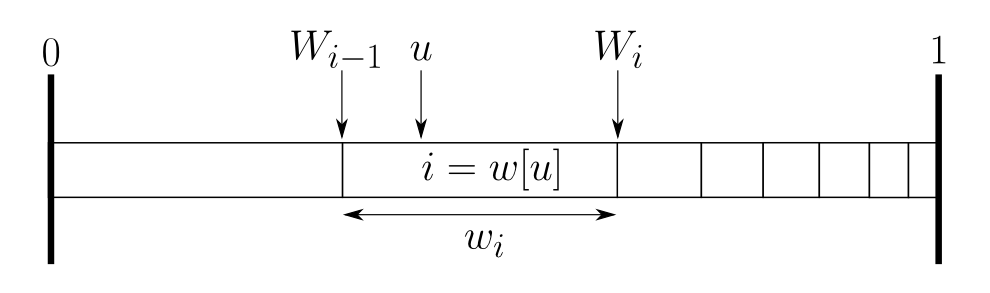
\includegraphics[width=0.9\columnwidth]{figures/pt2/mc_representation}
		\caption{Schematic representation of a Monte-Carlo computation}
		\label{fig:mc_representation}
Values inside the boxes are sample indices. Values outside are probabilities and drawn random numbers.

Drawing the random number $u$ with the partition function $w$ yields sample index $i=w[u]$
	\end{center}
\end{figure}




\section{The sample space}

\paragraph{``Sample'' and ``Comb''}
Because of its original nature, this algorithm casts some ambiguity on what should be refered to as a ``sample''. We are going to estimate a sum of elementary contributions $e_I$, compute and store them individually, and draw them based on a partition function ; therefore they will be refered to as the \emph{samples} and shown as such in the previously introduced representation. But the actual sample values ($s_i$ in the previous section) are sums over several $e_I$, refered to as \emph{combs}.


\paragraph{$C_I^2$ is used as a partition function}
Generator determinants are sorted with decreasing absolute values of $C_I$.
	As can be seen in figure \ref{fig:ei}, the values of $e_I$ span many orders of magnitude and decrease rapidly with $I$, in an exponential-looking way. Smoothed values for $e_I$ are shown in figure \ref{fig:p_i}. There are a few reasons for that.
\begin{itemize}
	\item
	The values for the denominator $\Delta E_\alpha$ used in the computation of $\epsilon(\alpha)$ tend to increase, as variational determinants tend to be more and more excited and to populate higher orbitals ( detailler ? )
	\item
	The number of unique $\ket \alpha$ per generator decreases. Indeed, the more ``previous generators'' there is, the likelier it is that a generated $\ket \alpha$ was generated before.
	\item
	Unique $\ket \alpha$ are, by construction, disconnected from all previous generators, which mean they connect to a smaller and smaller norm of $\Psi$ ( see figure \ref{fig:a_con} ). 
\end{itemize}


The last reason given for the decrease of $e_I$ is the most important one, and tells us that the most significant $\ket \alpha$ are those connecting to $\kI$, so the dominant terms of $e_I$ are 

\begin{equation}
\frac{C_I^2 \Hij{I}{\alpha}\Hij{\alpha}{I}}{\Delta E_{\alpha}}
\end{equation}

Consequently we chose

\begin{equation}
\tilde w_I = C_I^2
\end{equation}

as a partition function for $e_I$. This is however not the exact partition function used in the Monte-Carlo scheme. We will later introduce some slight modification to it, for algorithmic reasons.
As can be seen in figure \ref{fig:eici2}, $\frac{e_I}{C_I^2}$, which is very close to our sample space, indeed has a lower variance than $e_I$ but is still similar in that it spans orders of magnitude and overall decreases.

\section{Partition of the sample space}

\paragraph{Deterministic and stochastic ranges}
Because $e_I$ decreases rapidly, most of the contribution is contained in the first samples. We can compute the exact energy contribution for the first samples, and only make a stochastic estimation for the sum over the smaller ones. This effectively splits the sample space in two ranges, a deterministic one $\mathcal{D}$, then a stochastic one $\mathcal{S}$ (hence the hybrid characteristic of this method). Being ranges, they are always constituted(?) of contiguous samples. The estimated energy can be written as

\begin{equation}
\EPT = E_D + E_S
\end{equation}

with $E_D$ the exact energy for $\mathcal{D}$, and $E_S$ the estimated energy for $\mathcal{S}$. The error bar only applies to $E_S$, which typically much smaller than $E_D$.
The number of samples in $\mathcal{D}$ increases during the computation. Initially, $\mathcal{D}=\mathcal{T}_0$ the initial deterministic range, whose total weight is $u_0$.

\begin{equation}
\sum_{I \in \mathcal{T}_0} w_I=u_0
\end{equation}

$\mathcal{T}_0$ is always computed before any stochastic estimation can take place.

\paragraph{The stochastic range divided in $N_{teeth}$ \emph{teeth}}

Because $\frac{e_I}{w_I}$ overall decreases, a range has a lower variance than the whole set. The stochastic range is split in $N_{teeth}$ ranges refered to as \emph{teeth}, noted $\mathcal{T}_1,\ldots,\mathcal{T}_{N_{teeth}}$ and sharing the same total weight $W_T$

\begin{equation}
\sum_{I \in \mathcal{T}_{t \geq 1}} w_I=W_T
\end{equation}

The partition of the sample space is as follow

 \begin{figure}[h!]
	\begin{center}
		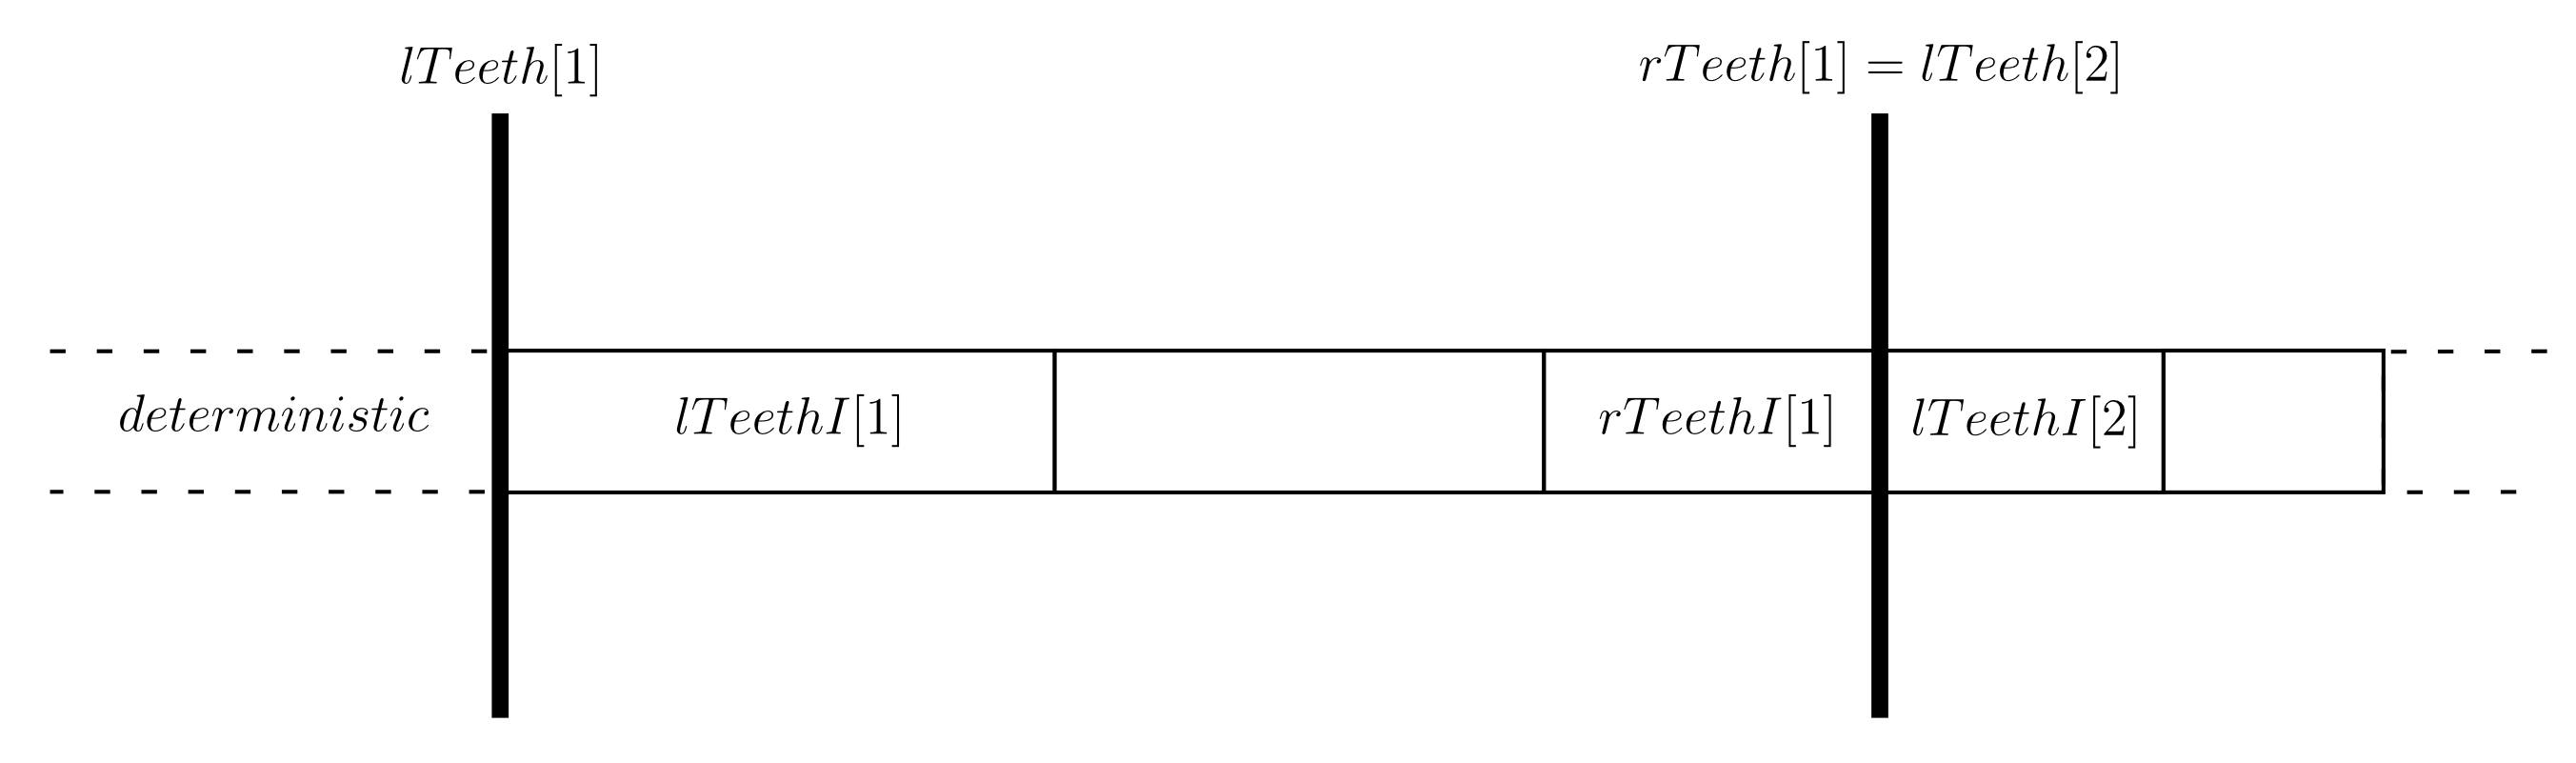
\includegraphics[width=0.9\columnwidth]{figures/pt2/teeth}
		\caption{Partitioning of the sample space}
		\label{fig:teeth}
		The sample space is partitioned in so-called \emph{teeth} from $\mathcal{T}_0$ to $\mathcal{T}_{N_{teeth}}$, $\mathcal{T}_0$ of total weight $u_0$, the others of total weight $W_T$
	\end{center}
\end{figure}

Intuitively, the sum of ``one large, one medium and one small'' has a lower variance than the sum of ``three at random''. Instead of drawing individual indices, we are going to draw ``combs'' of indices, which are correlated sets of 1 index from each tooth. The associated sample value is the sum of $\frac{e_I}{w_I}$ over those indices that are in $\mathcal{S}$.  The expression for this sample value is given as equation \ref{eq:combvalue}

\paragraph{fully-computed teeth are moved to the deterministic range}

Remembering we store $e_I$, given the first tooth $\mathcal{T}_t$ that contains an unknown $e_I$, the deterministic range extends to all $\mathcal{T}_{p<t}$. This makes $\mathcal{T}_t$ the first non-deterministic tooth.
The number or samples in the deterministic range, therefore, is function of a tooth index $t$, and noted $n_0(t)$, as seen in figure XXXXXXXXXX.


 \begin{figure}[h!]
	\begin{center}
		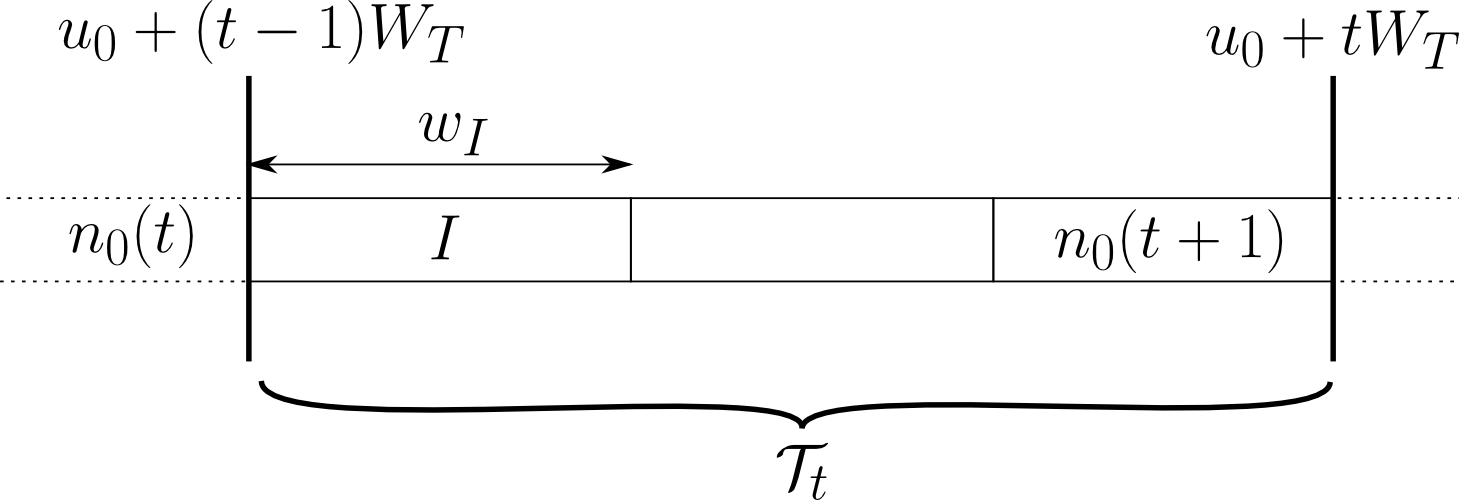
\includegraphics[width=0.9\columnwidth]{figures/pt2/tooththreshold}
		\caption{Boundaries of a teeth index-wise and probability-wise}
		\label{fig:teeth}
		
	\end{center}
\end{figure}


\paragraph{comb values}

We can write the expression of $B_t(u)$ the sample value associated with a comb. It is function of a randow number $u \in [0,1)_\mathbb{R}$ and $t$ the index of the first non-deterministic tooth.

\begin{align}
\label{eq:combvalue}
B_t(u) = W_T \sum_{i=t-1}^{N_{teeth}-1} \frac{e_{y(u+i)}}{w_{y(u+i)}} \\
y(x)=w[u_0+ W_T \times x, W]
\end{align}
\alert{merite sans doute plus d'explications...}

An illustrative exemple is given as figure \ref{fig:toothindet}.

 \begin{figure}[h!]
	\begin{center}
		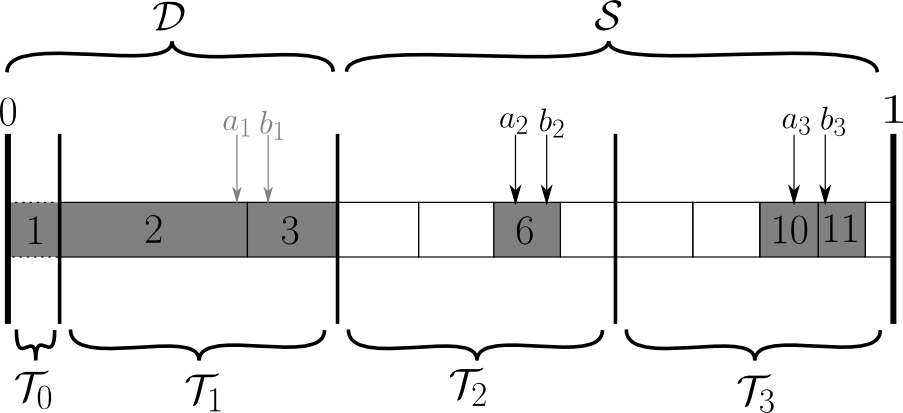
\includegraphics[width=0.9\columnwidth]{figures/pt2/toothindet}
		\caption{illustrative example of drawing two combs $a$ and $b$}
		\label{fig:toothindet}
		Samples that have been computed are greyed. $\mathcal{T}_1$ has been fully computed and is thus moved to $\mathcal{D}$. The first non-deterministic/not fully-computed tooth is $\mathcal{T}_2$.
		$$E_D = e_1 + e_2 + e_3$$
		$$B_2(a) = \frac{e_6}{w_6} + \frac{e_{10}}{w_{10}}\;;B_2(b) = \frac{e_6}{w_6} + \frac{e_{11}}{w_{11}}$$
		$$E_S = \frac{B_2(a)+B_2(b)}{2} \times W_T \alert {A CHECK}$$
	\end{center}
\end{figure}

\paragraph{estimation of $\EPT$}

After drawing $n$ random numbers forming the set $\mathcal{U}$, and given $\mathcal{T}_t$ the first non-deterministic tooth, $\EPT$ can be estimated as 

\alert{A VERIFIERXXXXXXXXXXXXXXXXXXXXXXXX}
\begin{equation}
\sqrt{(S_{t}^{(2)} - S_{t}) n^{-1} }
\end{equation}		

\begin{align}
 S_{t} = \sum_{u \in \{\mathcal{U}\}_n} B_{t}(u) \\
 S^{(2)}_{t} = \sum_{u \in \{\mathcal{U}\}_n} B_{t}(u)^2
\end{align}




\section{Technical considerations}


\subsection*{why an initial deterministic part?}

The initial deterministic range $\mathcal{T}_0$ is a technical constraint.

Because samples are sorted with decreasing $\tilde w_i$, it is guaranteed that $|\mathcal{T}_{t>t'}| \geq |\mathcal{T}_{t'>0}|-1$.
For each comb, we draw a sample in each teeth, and when a tooth is entirely computed, it is moved to $\mathcal{D}$. Thus, it is immediately obvious that a tooth containing a single sample makes no sense, as it will be instantly moved to $\mathcal{D}$ ; it can as well be considered part of it. Because it's usually accepted (???) that it takes at least 30 samples to estimate a variance, we can go further and consider that a tooth with fewer than 5-10 samples will be moved to $\mathcal{D}$ too fast to be of real interest. Because the first $C_I^2$ are usually disproportionately large, it's not possible to fit that many in a tooth. Therefore they are immediately considered part of $\mathcal{D}$.

\subsection*{desired \textit{vs} effective partition function}

We have defined all teeth (except the special $\mathcal{T}_0$) as sharing the same total weight $W_T$. This is a constraint on our desired partition function $\tilde w_I = C_I^2$ that will lead to the effective partition function $w_I$.

We are sampling comb values, but we have defined $\tilde w_I$ a partition function for $e_I$. Since we impose that the same number of $e_I$ are drawn in each tooth - one per comb - the relative weight of teeth becomes irrelevant, and we effectively give all teeth the same weight 
\begin{equation}
W_T=\frac{1-u_0}{N_{teeth}}
\end{equation}
in the Monte-Carlo scheme. Therefore, the effective weight given to $e_I \in \mathcal{T}_t$ is

\begin{equation}
w_{I \in \mathcal{T}_t} = W_T \times \frac{\tilde w_I}{\sum_{J \in \mathcal{T}_t} \tilde w_J}
\end{equation}

To leave the partition function unaltered, we need all teeth to actually weight $W_T$

\begin{equation}
\sum_{J \in \mathcal{T}_t} \tilde w_J = W_T
\end{equation}

Clearly this is not going to be the case for any reartition function $\tilde w$. Schematically, as seen in figure \ref{fig:toothbuilding}, it would require the threshold between two teeth to exactly match the threshold between two samples. It is possible to artificially split a sample to get a matching threshold, but this adds some complexity implementationally speaking.

We have enforced that all teeth contain at least 5-10 samples - and they usualy contain a lot more, up to hundreds of thousands. Therefore, a simpler solution is to ``round'' the teeth thresholds to the $e_I$ threshold directly above, which will result in teeth with weights close to $W_T$, and thus the effective partition function will be little different from the desired one. Since our partition function is an extremely rough estimation of $e_I$, this is unlikely to cause any significant change in convergence speed.

Essentially, we will use $\tilde w$ only to define the $\mathcal{T}_t$ sets, then use $w$ as the actual partition function. This gives us, by definition, teeth weighting exactly $W_T$.
This is illustrated in figure \ref{fig:toothbuilding}.
 
 \begin{figure}[h!]
	\begin{center}
		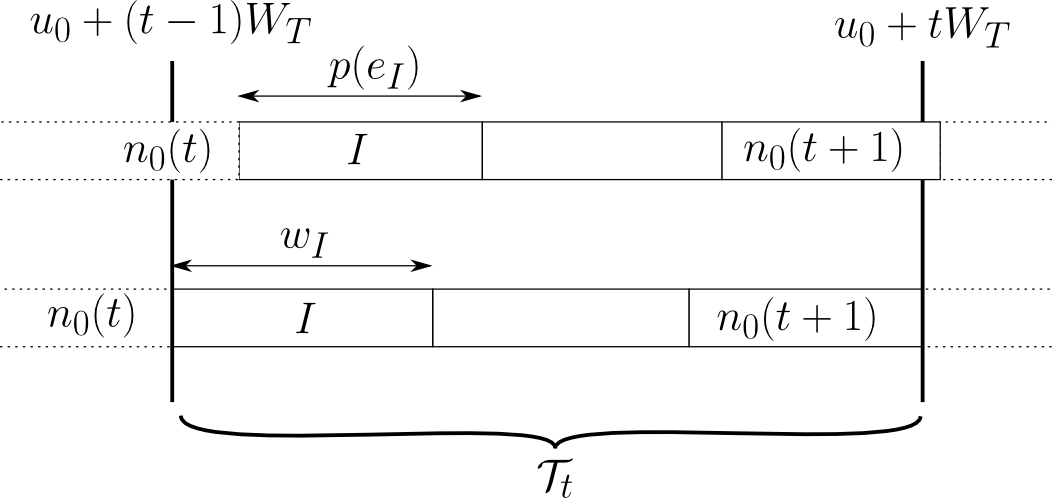
\includegraphics[width=0.9\columnwidth]{figures/pt2/toothbuilding}
		\caption{Adjusting sample weights}
		\label{fig:toothbuilding}
		 Desired weights $\tilde w_i$ are adjusted to effective weights $w_i$ so as to satisfy
		 $$\sum_{I \in \mathcal{T}_n} w_I = W_T$$
	\end{center}
\end{figure}





\subsection*{tooth filling}

This is an empirical mechanism to balance the stochastic and deterministic aspect of this method. For a tooth containing $n$ samples of equal weight, full computation is acheived after on average (A VERIFXXXXXXXXXXXXXXXXXXXXXXX)

\begin{equation}
\sum_{i=0}^{n-1} \frac{n}{n-i}
\end{equation}

combs are drawn. Thus, teeth containing thousands of determinants are very hard to move to $\mathcal{D}$. A tooth containing 10000 samples with a single uncomputed one, only needs computation that sample to be moved to $\mathcal{D}$, but it will take on average 10000 more combs to be drawn until this happens by chance.
A convenient way to avoid this frustrating situation is, everytime a comb is drawn, to additionally compute the first uncomputed sample of the whole space. This ensures smooth filling of teeth, and that that the full deterministic computation will be achieved before $\Ngen$ combs are drawn.

\section{implementation}


\subsection{drawing}

The algorithm to find a sample index associated with drawing $u$ in with a partition function $w$ is show as algorithm \ref{alg:FIND_SAMPLE}.

\begin{algorithm}
\label{alg:FIND_SAMPLE}
\caption{FIND\_SAMPLE}
\SetKwFunction{FFind}{FIND\_SAMPLE}
	\SetKwProg{Fn}{Function}{:}{}
	
	\Fn(\tcc*[h!]{Finds sample index associated with drawing random value $v$ in a cumulative probability distribution $p$}){\FFind{$v$,$p$}}{
		\KwData{$0 \leq v < 1$}
		\KwData{$p$ float array of size $N$ with $p[0]=0$, $p[N]=1$, $p[n+1] \geq p[n]$}
		\KwResult{Returns $i$ so that $p[i-1] \leq v < p[i]$}
		
		\tcc {The result must be in the range $[l,r]_\mathbb{Z}$. We set them for the most general case}
		$l \gets 0$ \;
		$r \gets N$ \;
		
		\While{$r-l > 1$}{
			$i \gets \lfloor (r+l) / 2 \rfloor$ \;
			\uIf{$p[i] < v$}{
				$l \gets i$ \;
			}
			\Else{
				$r \gets i$ \;
			}
		}
		\KwRet $r$ \;
	}
\end{algorithm}




\subsection{building teeth}

\begin{itemize}

\item
\emph{input}
\begin{description}
\item[$\tilde w_I$]
The desired partition function, which we chose to be $C_I^2$.
\item[$\Nteeth$]
A desired number of teeth
\item[$\minDetInT > 1$]
A desired minimal number of samples in first teeth. All subsequent teeth are guaranteed to contain $\minDetInT-1$ samples.
\end{description}

\item
\emph{output}
\begin{description}
\item[$w_I$]
The effective partition function
\item[$n_0(t)$]
An array of size $\Nteeth+1$ so that $n_0(t)$ is the number of samples in $\mathcal{D}$ with $\mathcal{T}_t$ the first non-deterministic tooth. For algorithmic convencience, $n_0(\Nteeth+1)=\Ngen$.
\end{description}
\end{itemize}


There is no trivial way to ensure teeth building will succeed with a given set of parameters. 
With $n_0(1)$ the size of the initial deterministic set $\mathcal{T}_0$, teeth building is sure to fail if 
\begin{equation}
\Ngen - n_0(1) < \minDetInT \times \Nteeth
\end{equation}
However, it may not succeed as there is no guarantee the first tooth will contain $\minDetInT$ samples. Because samples are sorted with decreasing $\tilde w_I$, each tooth is guaranteed to contains as many or more samples than the previous one, so we only need to ensure $|\mathcal{T}_1| \geq \minDetInT$.
Relying on the fact that relative values of $\tilde w_I$ get closer and closer, we increment $n_0(1)$ until either the first tooth contains enough samples, or the impossibility condition is reached.

\begin{algorithm}
	\caption{COMPUTE\_TEETH}
	$\tilde W_I = \sum_{i \leq I} {\tilde w_i}$ \;
	$n_0(1) \gets 0$ \;

	\While{}{
		$u_0 \gets \tilde W[n_0(1)]$\;
		$r \gets \tilde W[n_0(1)+\minDetInT]$ \;
		$W_T = \frac{1 - u_0}{N_{teeth}}$ \;
		\If{$W_T \geq r - u_0$}{
			break loop\;
		}
		
		$n_0(1) \gets n_0(1) + 1$ \;
		\If{$\Ngen - n_0(1) < \minDetInT \times \Nteeth$}{
			\tcc{cannot compute with those parameters} \;
			try with fewer teeth \;
		}

	}
\end{algorithm}

Then, $n_0(t)$ can be fully computed

\begin{algorithm}
	\caption{COMPUTE\_TEETH}
	\For{$t=2,N_{teeth}$}{
		$r = u_0 + W_T \times (t-1)$ \;
		$n_0(t) = FIND\_SAMPLE(r, \tilde W)$ \;
	}
	$n_0(\Nteeth+1) = \Ngen$ \;
\end{algorithm}

%$n_0(\Nteeth)$ has to be treated separately, as by construction $u_0 + \Nteeth W_T = 1$, which is outside of the range $[0,1)_\mathbb{R}$ defined for $u$ in FIND\_SAMPLE.

And the effective partition function $w_I$

\begin{algorithm}
	\caption{COMPUTE\_TEETH}
	$w_{i<n_0(1)} \gets \tilde w_{i<n_0}$ \;
	\For{$t=1,N_{teeth}$}{
		$\text{tooth\_width} = \tilde W_{n_0(t+1)} - \tilde W_{n_0(t)}$ \;
		\For{$i=n_0(t)+1, n_0(t+1)$}{
		$w_{i} = \tilde w_{i} \times \frac{W_T}{\text{tooth\_width}}$ \;
		}
	}
	
\end{algorithm}



\subsection{Building task queue}

For a massively parallel implementation, we need to create a task queue. Because values for $e_I$ are stored, quite clearly, we need one task per generator determinant. Because of the tooth filling mechanism, we know we will need at most $\Ngen$ combs.
\begin{description}
\item{$J$} is the task queue, $J[i]$ the index of the $i^{th}$ sample $e_I$ that must be computed.
\item{$d$} keeps track of the computed samples. $d[I] = TRUE$ iff $e_I$ has already been computed.
\item{$N_j$} is the number of tasks currently created. When the task queue is fully computed $N_j = \Ngen$.
\item{$N_c$} is the number of combs currently drawn.
\item{$R$} is an array of integer size $\Ngen$, keeping track of available combs at any point of the computation. The collector node checks $R[j]$ when the first $j$ tasks have been computed (for all $j$ with increasing order). If $R[j] = c \neq 0$, all samples for comb $c$ have just become available. 
\end{description}



\begin{algorithm}
	$R \gets $ array size $\Ngen$ initialized to 0 \;
	$N_c \gets 0$ \;
	$N_j \gets n_0(1)$ \;
	
	\For{$i=1,n_0(1)$}{
		$d[i] \gets TRUE$ \;
		$J[i] \gets i$ \;
	}
	
	\For{$i=1,\Ngen$}{
		$u[i] \gets $ random value in $[0,1)_\mathbb{R}$ \;	
	}
	$F \gets 0$ \;	
	\While{$N_j < \Ngen$}{
  	ADD\_COMB  shown as algorithm \ref{alg:ADD_COMB}\;
	$R[N_j] \gets N_c$ \;
	FILL\_TOOTH shown as algorithm \ref{alg:FILL_TOOTH} \;
	}
	\tcc{for convenience, makes sure the last task matches the last comb, rather than a tooth filling}
	\If{$\Ngen > 1$}{
		$R[N_j-1] \gets 0$ \;
		$R[N_j] \gets N_c$ \;
	}
\end{algorithm}

\begin{algorithm}
	\caption{ADD\_COMB}
	\label{alg:ADD_COMB}
		\KwData{$N_c,u[N_c],F,d,N_j,J$ as in the namespace of the calling function}
		\KwData{$\tilde M$ as in the namespace of the calling function if defined, otherwise ignored}
		$N_c \gets N_c + 1$ \;
  		\For{$t=0,N_{teeth}-1$}{
		%$v \gets lTeeth[t] + rand \times toothSize[t]$ \;
		$v \gets u_0 + W_T \times (t+u[N_c])$ \;
		
		%$i=FIND\_SAMPLE(rand, lTeethI[t], rTeethI[t])$ \;
		$i=FIND\_SAMPLE(v, W)$ \;
		$\tilde M_i \gets \tilde M_i + 1$ \;
		\If{$not\ d[i]$}{
			$N_j \gets N_j + 1$ \;
			$J[N_j] \gets i$ \;
			$d[i] \gets TRUE$ \;
		}
	}
\end{algorithm}

\begin{algorithm}
	\caption{FILL\_TOOTH}
	\label{alg:FILL_TOOTH}
	\KwData{$F$,$d$,$N_j$,$J$ as in the namespace of the calling function}
	
	\While{$F < \Ngen$}{
   		$F \gets F + 1$ \;
       \If{$not\ d[F]$}{
          $N_j \gets N_j+1$ \;
          $J[N_j] \gets F$ \;
          $d[F] \gets TRUE$ \;
          break \;
        }
	}
\end{algorithm}

\subsection{computing estimation and error}


\begin{algorithm}
	$n \gets 1$ \;
	$t \gets 0$ \;
	$U \gets 0$ \;
	$f$ integer array size $\Ngen$ initialized with $F$ the fragmentation. \;
	$d$ logical array size $\Ngen+1$ initialized with FALSE \;
	$S$ and $S^{(2)}$ float arrays size $\Nteeth+1$ initialized with $0$ \;
	\While{$n \leq N_{gen}$}{
		\uIf{$f[J[n]] = 0$}{
			$d[J[n]] = true$ \;
			\While{$d[U+1]$}{
				$U \gets U + 1$ \;
			}
			\tcc{shortcut boolean evaluation required to prevent out of bound access to $n_0$}
			\While{$t \leq \Nteeth \wedge U \geq n_0(t+1)$}{
				$t \gets t+1$ \;
				$E_0 \gets \sum_{I<n_0(t)} e_I$ \;
			}
			\If{$R[n] \neq 0$}{
				$c \gets R[n]$ \;
				$S_* \gets S_* + B_*(u[c])$ \;
				$S^{(2)}_* \gets S^{(2)}_* + B_*(u[c])^2$ \;
				$E \gets E_0 + S_t/c$ \;
				error $\gets \sqrt{(S_t^{(2)} - {S_t}^2)(c-1)^{-1} }$ \;
				exit on acceptable error \;
			}
			$n \gets n+1$ \;
		}
		\Else{
			retrieve $I$ and $e_I$ \;
			store $e_I$ \;
			$f[I] \gets f[I]-1$ \;
		}
	}
	\tcc{estimated energy $E \pm \text{error}$}
\end{algorithm}


\begin{algorithm}
	\tcc{efficiently computes $S_* \gets S_* + B_*(u)$  and $S^{(2)}_* \gets S^{(2)}_* + B_*(u)^2$}
	
					
	$x \gets 0$ \;
	\For{$t=N_{teeth},1,-1$}{
		$I \gets FIND\_SAMPLE(u_0+W_T \times (u+t-1), W)$ \;
		$x \gets x + W_T \times \frac{e_{I}}{w_I}$ \;
		$S_t \gets S_t + x$ \;
		$S^{(2)}_t \gets S^{(2)}_t + x^{2}$ \;
	}
\end{algorithm}




\begin{figure}[h!]
	\begin{center}
		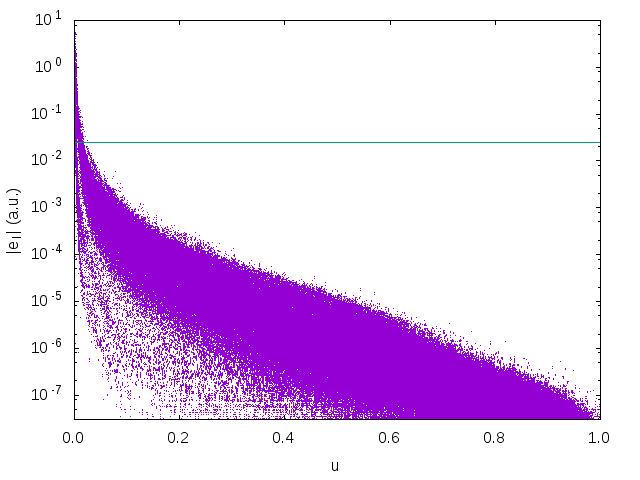
\includegraphics[width=0.9\columnwidth]{figures/pt2/eI}
		\caption{A REFAIRE NOTATION.............}
		\label{fig:ei}
		$e_I$
	\end{center}
\end{figure}

\begin{figure}[h!]
	\begin{center}
		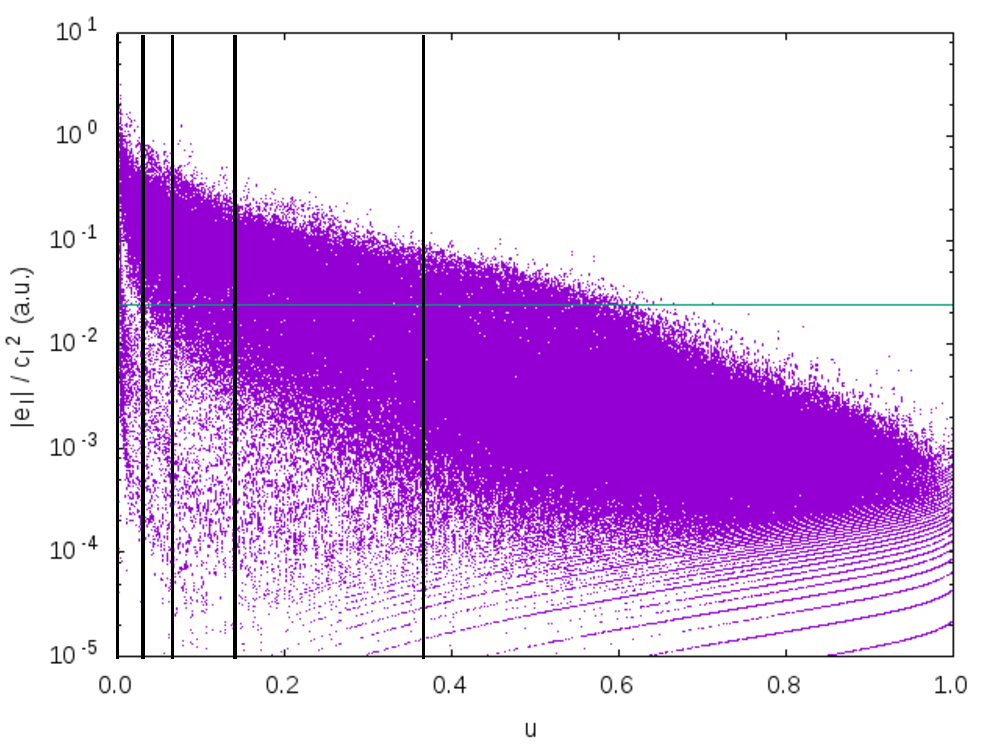
\includegraphics[width=0.9\columnwidth]{figures/pt2/eici2comb}
		\caption{A REFAIRE NOTATION.............}
		\label{fig:eici2comb}
		$e_I$
	\end{center}
\end{figure}



\begin{figure}[h!]
	\begin{center}
		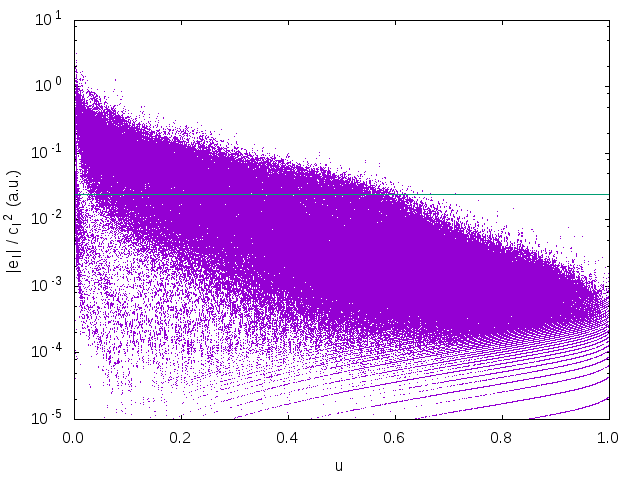
\includegraphics[width=0.9\columnwidth]{figures/pt2/eici2}
		\caption{A REFAIRE NOTATION.............}
		\label{fig:eici2}
		$e_I$
	\end{center}
\end{figure}


\begin{figure}[h!]
	\begin{center}
		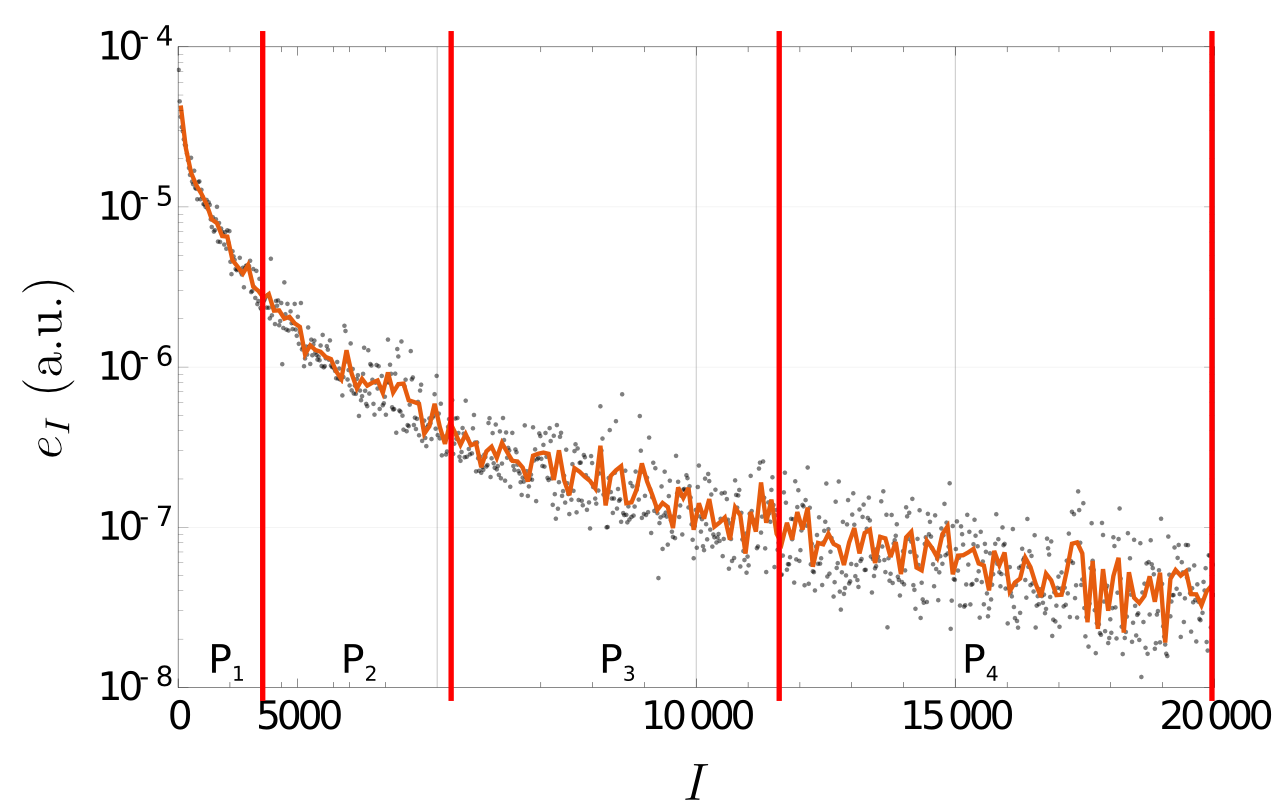
\includegraphics[width=0.9\columnwidth]{figures/pt2/P_i}
		\caption{A REFAIRE NOTATION.............}
		\label{fig:p_i}
		$e_I$
	\end{center}
\end{figure}



\begin{figure}[h!]
	\begin{center}
		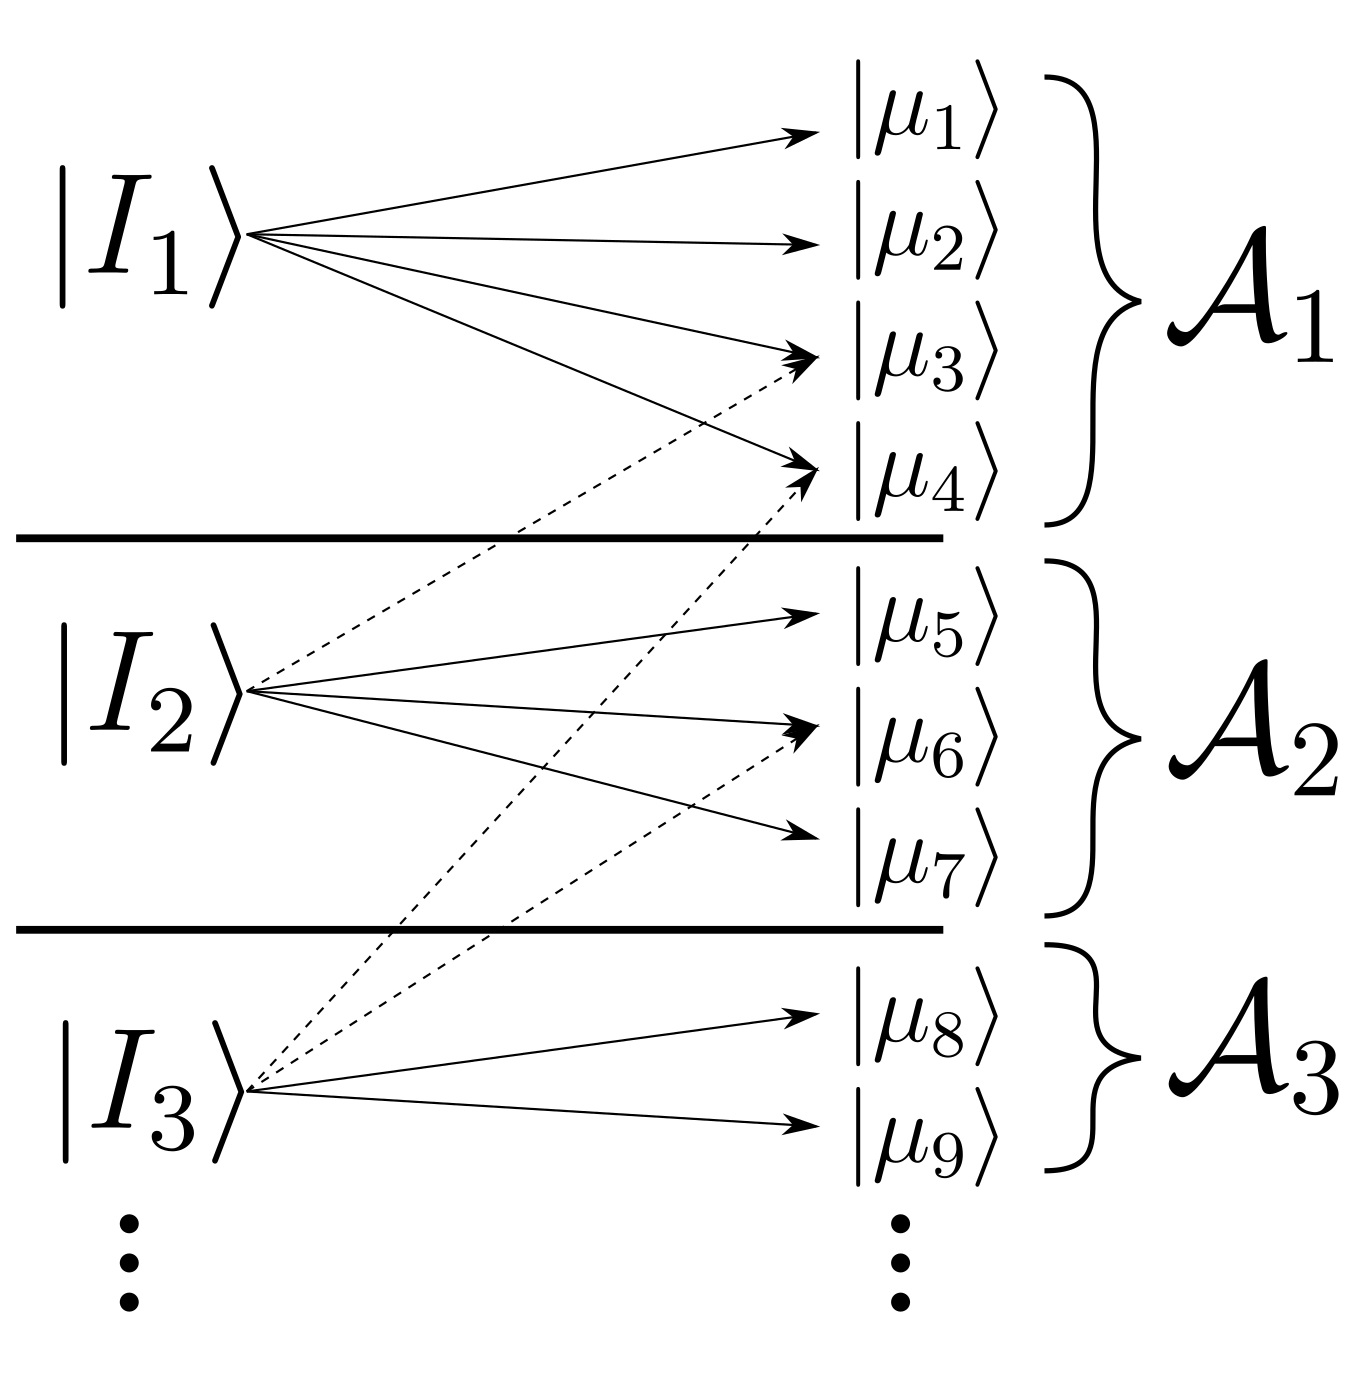
\includegraphics[width=0.5\columnwidth]{figures/pt2/mu_sample}
		\caption{}
		\label{fig:mu_sample}
		Construction of batches of $\ket \alpha$
	\end{center}
\end{figure}


\end{document}


